% En este apendice incluimos imágenes de mayor tamaño que no caben en el cuerpo del documento.

Este apéndice contiene imágenes de mayor tamaño que no caben en el cuerpo del documento. Algunas imágenes son versiones ampliadas de las imágenes que se han mostrado en el cuerpo del documento, otras son imágenes adicionales que no se han mostrado en el cuerpo del documento. En la tabla \ref{tab:larger_images} se puede ver una lista de las imágenes que se van a mostrar en este apéndice.

% Tabla indicando las imágenes adicionales que se van a mostrar en este apéndice
\begin{table}[H]
    \centering
    \begin{tabular}{|c|c|}
        \hline
        \textbf{Imagen} & \textbf{Descripción} \\ \hline
        \ref{fig:example_damage_types_large} & Ejemplos de los tipos de daños en el pavimento de la CRDDC2022. \\ \hline
        \ref{fig:datasetNinja_class_count_bar_large} & Número de anotaciones por clase en los datos de la CRDDC2022. \\ \hline
        \ref{fig:example_images_region_large} & Ejemplos de imágenes de los datos de la CRDDC2022. \\ \hline
        \ref{fig:ground_truth_examples_large} &  Ejemplos de comparación entre el ground truth y las detecciones del modelo. \\ \hline
    \end{tabular}
    \caption{Imágenes adicionales mostradas en este apéndice.}
    \label{tab:larger_images}
\end{table}
\newpage

% Añadimos img/example_damage_types_grid.png en tamaño grande ocupando toda la página en horizontal
\begin{figure}
    \centering
    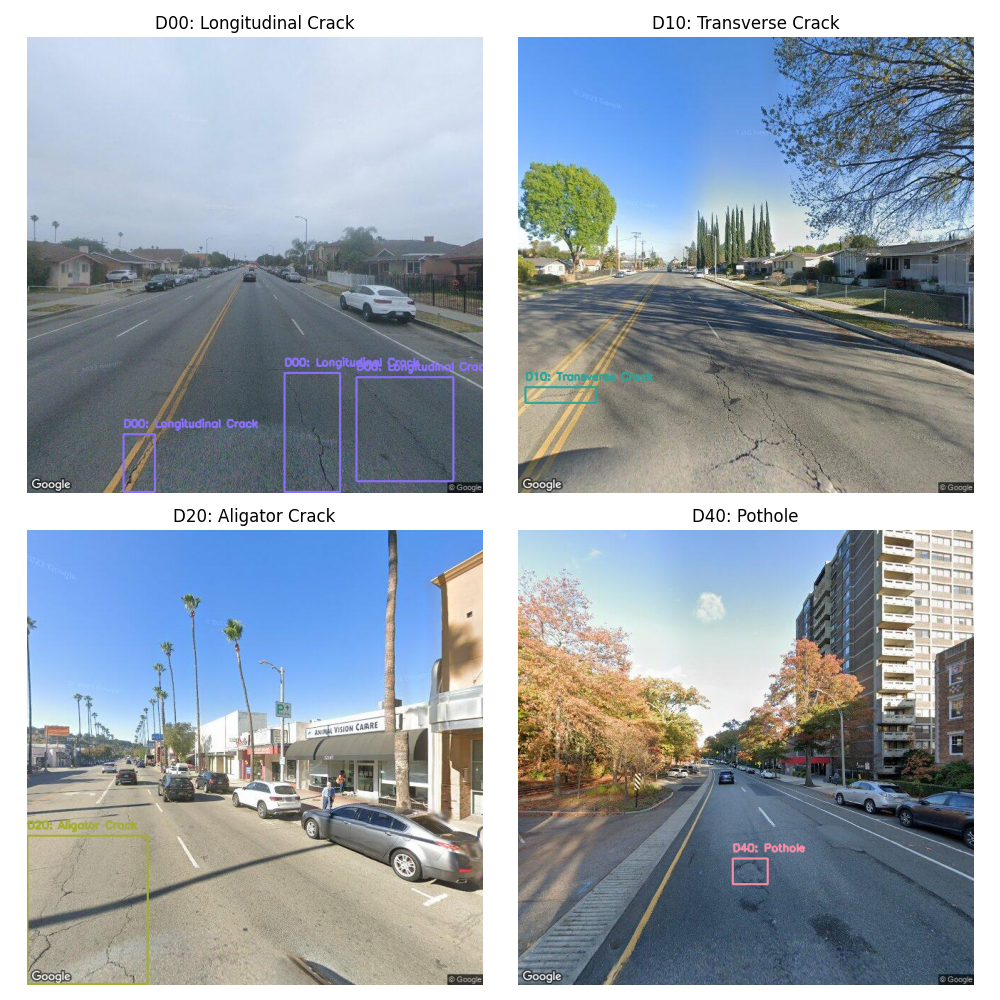
\includegraphics[width=\textwidth,height=\textheight,keepaspectratio]{img/example_damage_types_grid.png}
    \caption{Ejemplos de los tipos de daños en el pavimento de la CRDDC2022. Solo se han marcado los daños en el pavimento correspondientes a la clase que se quiere mostrar.}
    \label{fig:example_damage_types_large}
\end{figure}

% Añadimos figura con ../graphs/datasetNinja_class_count_bar.png y ../graphs/datasetNinja_class_count_by_region_bar.png en tamaño grande ocupando toda la página en vertical
\begin{figure}
    \centering
    \subfigure[Numero de anotaciones por clase]{
        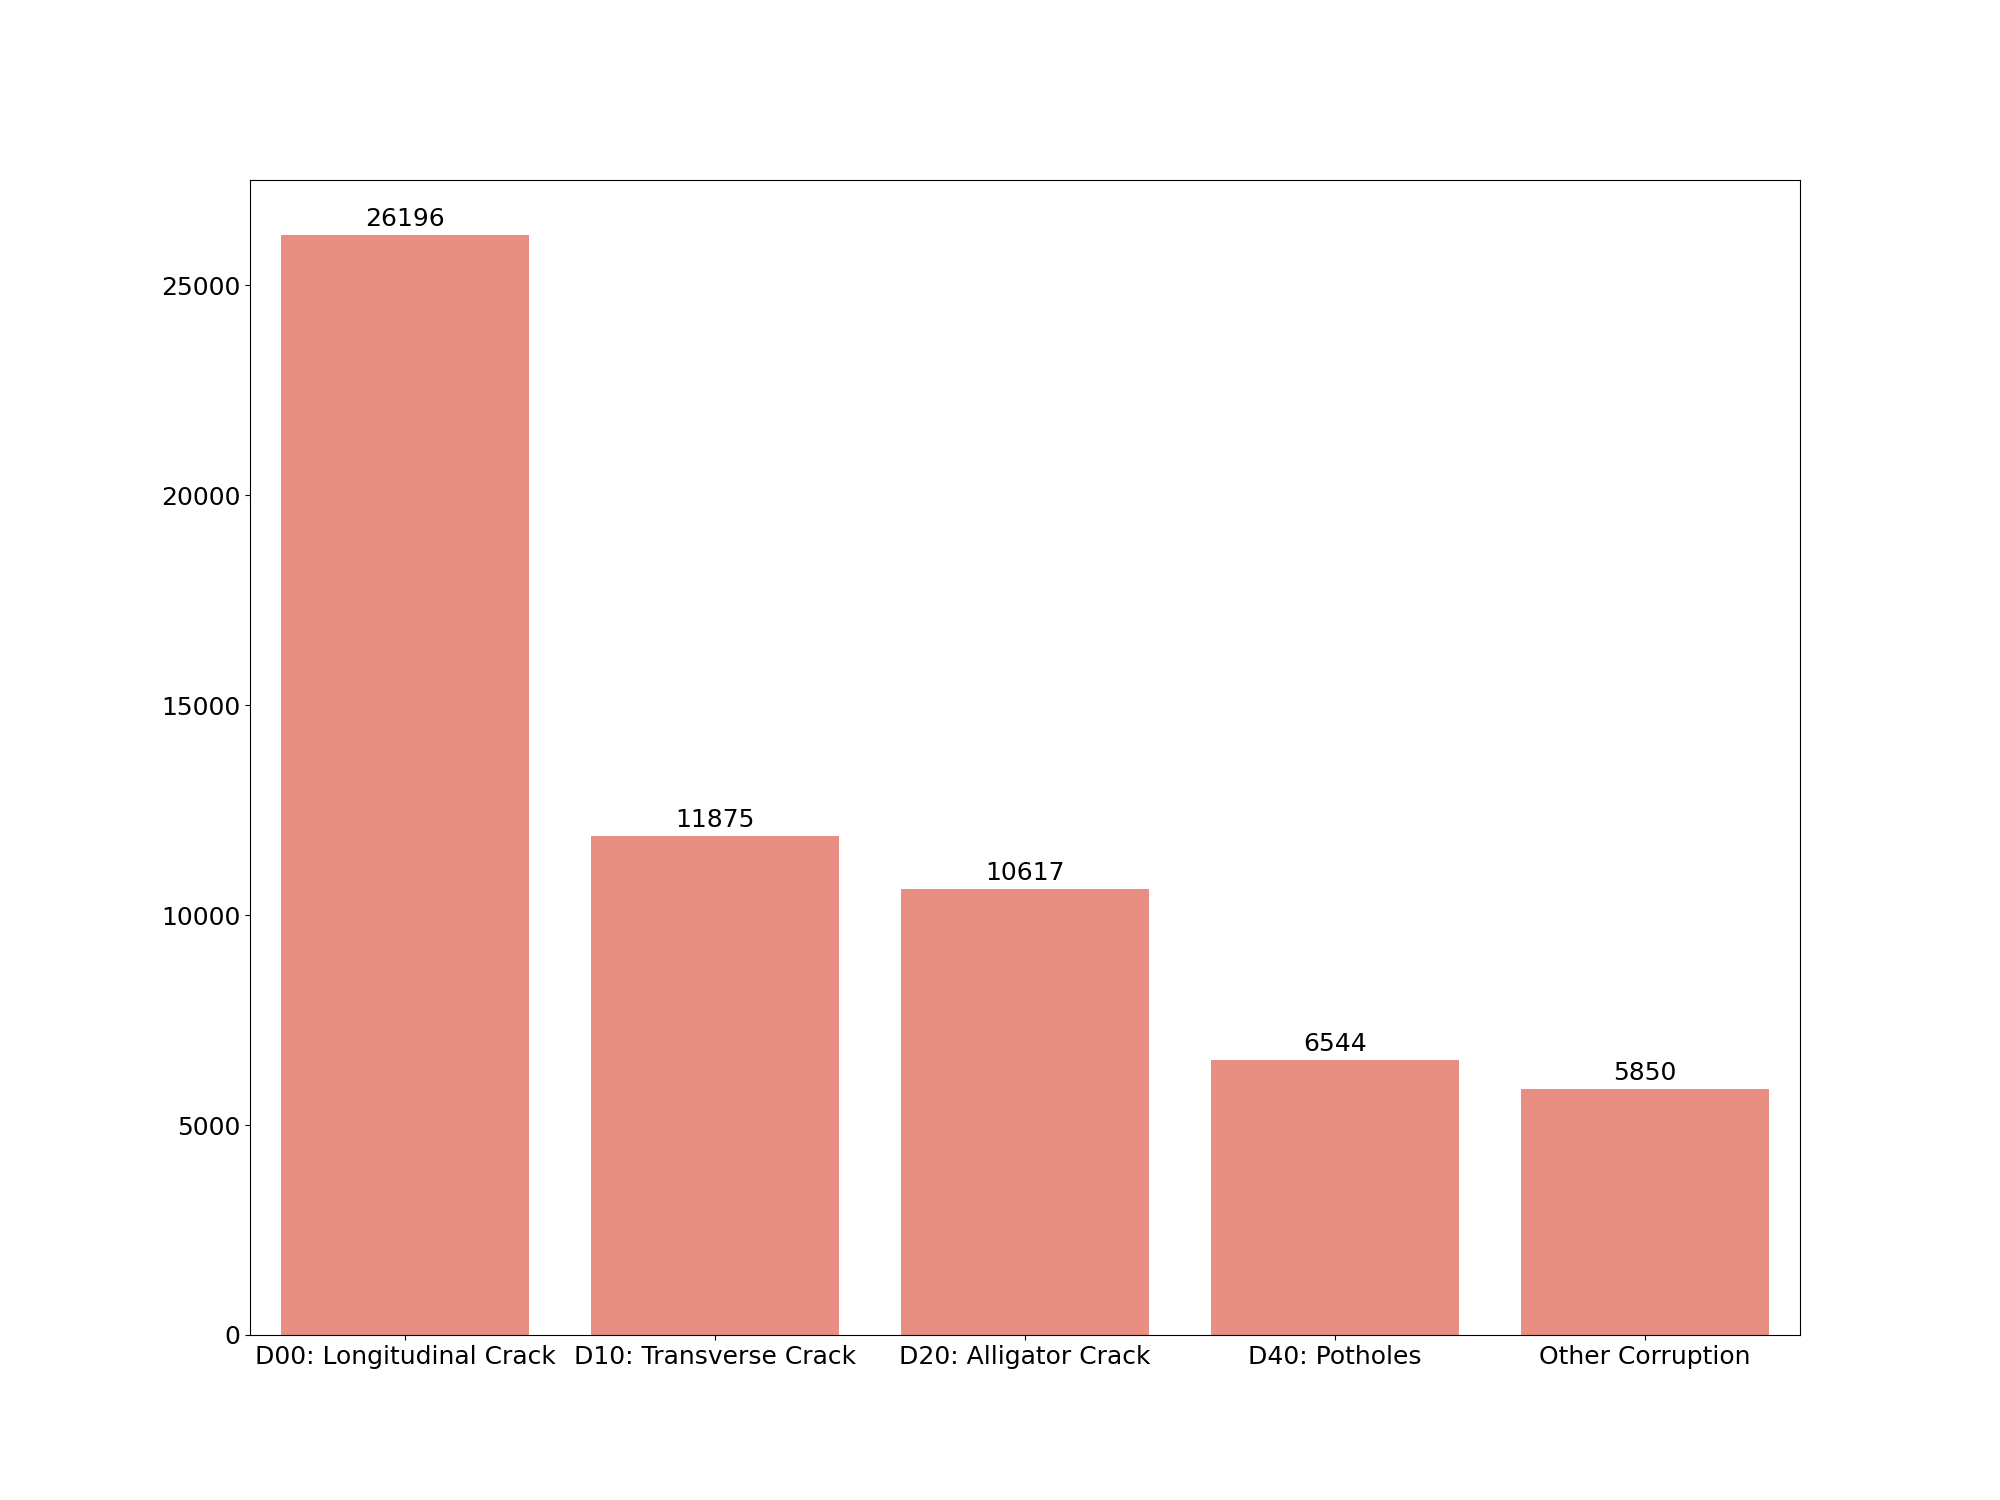
\includegraphics[width=0.9\textwidth]{../graphs/datasetNinja_class_count_bar.png}
        \label{fig:datasetNinja_class_count_bar_subfig1}
    }
    \subfigure[Numero de anotaciones por clase y región]{
        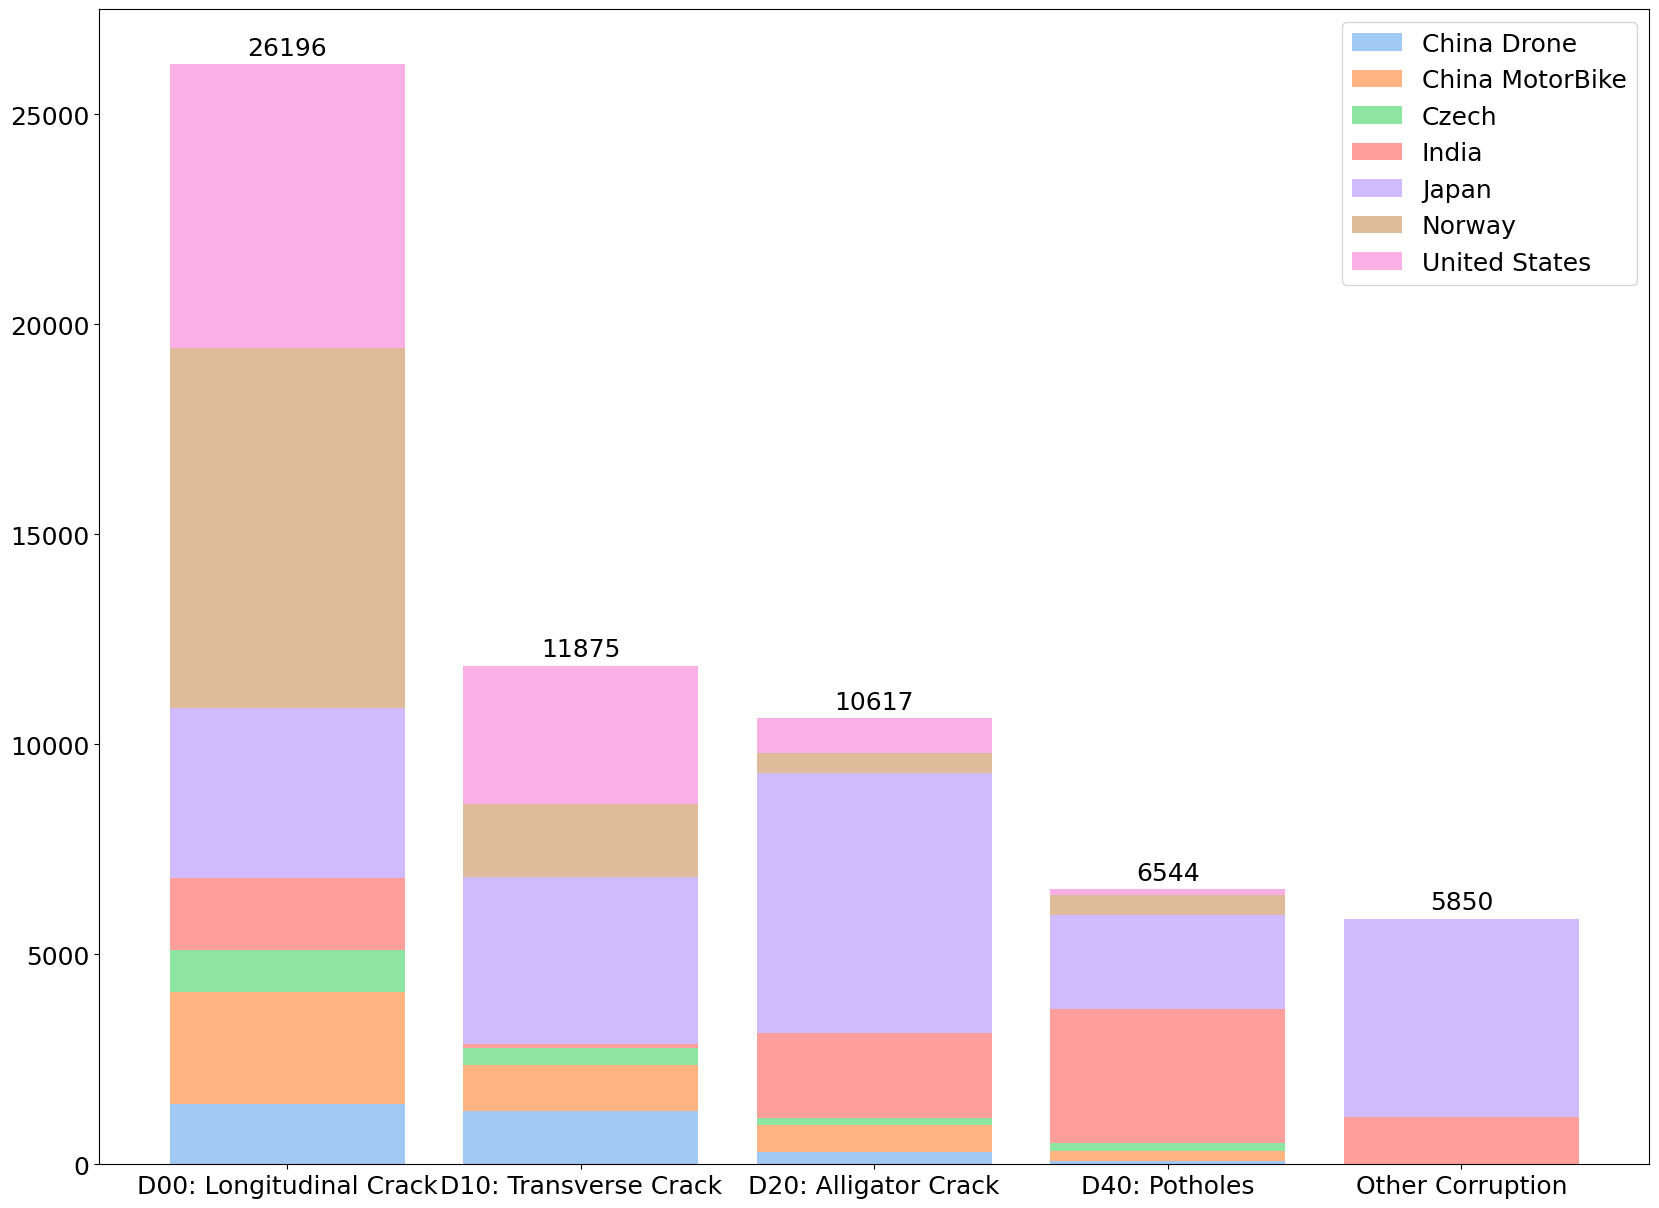
\includegraphics[width=0.9\textwidth]{../graphs/datasetNinja_class_count_by_region_bar.png}
        \label{fig:datasetNinja_class_count_bar_subfig2}
    }
    \caption{Número de anotaciones por clase en los datos de la CRDDC2022.}
    \label{fig:datasetNinja_class_count_bar_large}
\end{figure}

% Añadimos img/example_images_regions.png en tamaño grande ocupando toda la página en vertical
\begin{sidewaysfigure}
    \centering
    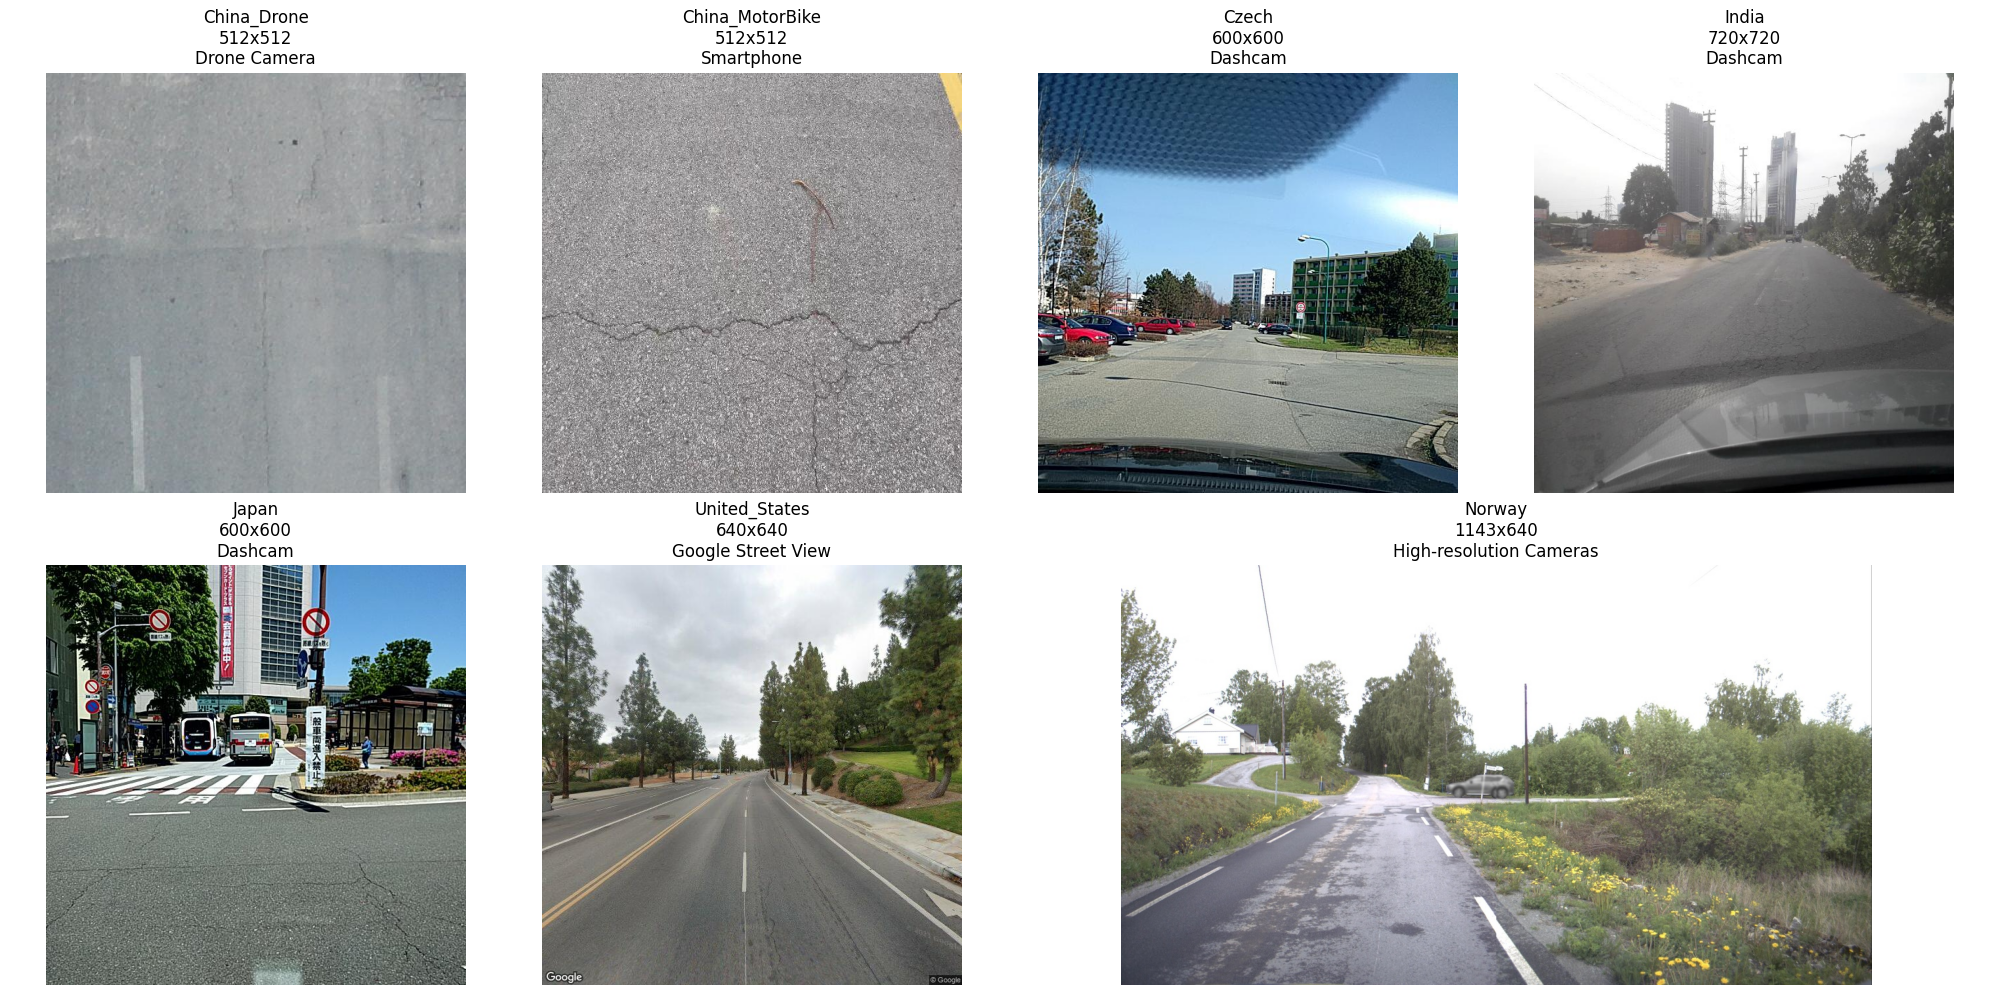
\includegraphics[height=\textheight,width=\textwidth,keepaspectratio]{img/example_images_regions.png}
    \caption{Ejemplos de imágenes de los datos de la CRDDC2022.}
    \label{fig:example_images_region_large}
\end{sidewaysfigure}

% Añadimos img/ground_truth_example_1.png y img/ground_truth_example_4.png
\begin{figure}
    \centering
    \subfigure[Ejemplo en el que al \textit{ground truth} le faltan anotaciones. A la derecha, se puede ver que el modelo ha detectado dos grietas longitudinales que no aparecen en el \textit{ground truth}.]{
        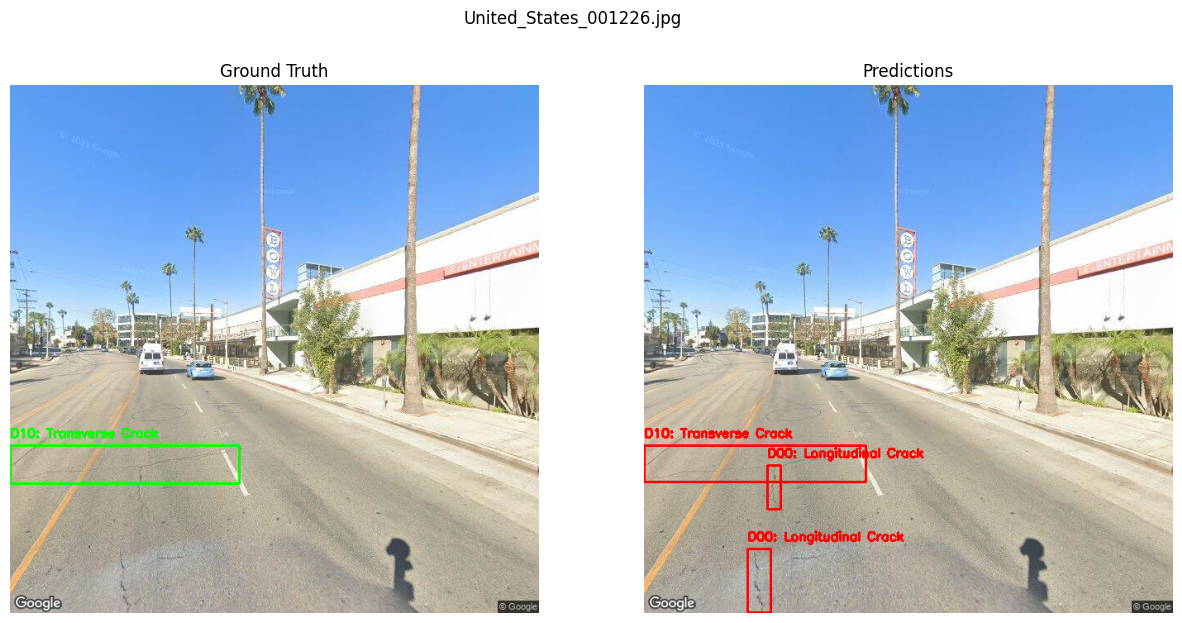
\includegraphics[width=1\textwidth]{img/ground_truth_example_1.png}
        \label{fig:ground_truth_example_1_large}
    }
    \vskip\baselineskip
    \subfigure[Ejemplo en el que el modelo genera varias anotaciones más pequeñas en lugar de una sola grande, como en el \textit{ground truth}.]{
        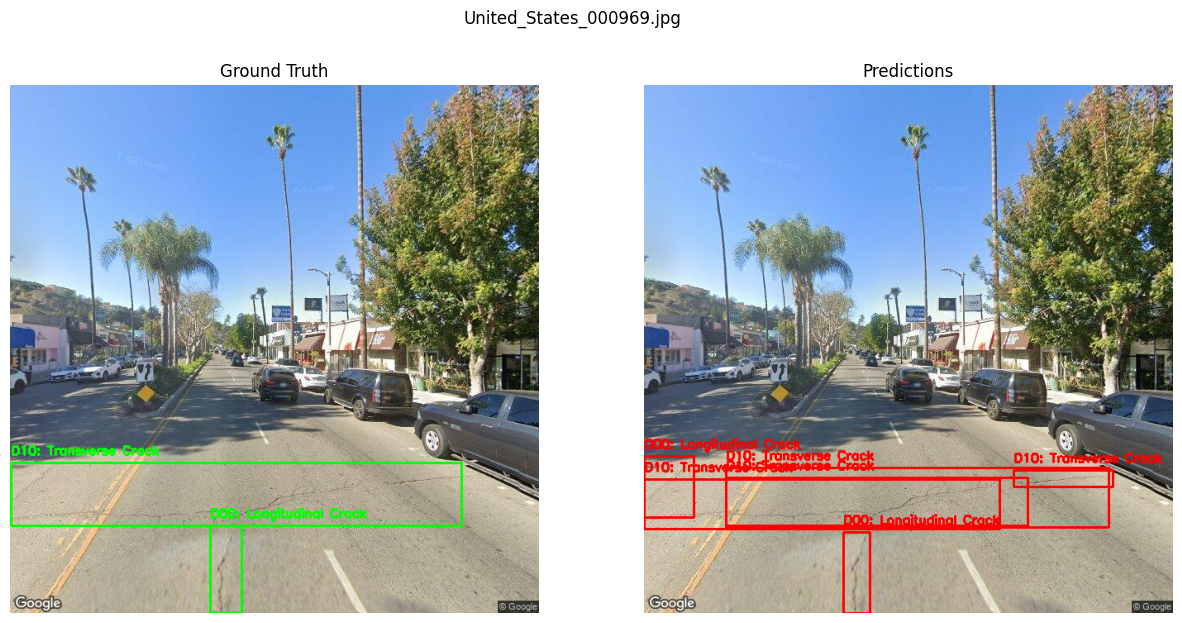
\includegraphics[width=1\textwidth]{img/ground_truth_example_4.png}
        \label{fig:ground_truth_example_4_large}
    }
    \caption{Ejemplos de comparación entre el \textit{ground truth} y las detecciones del modelo.}
    \label{fig:ground_truth_examples_large}
\end{figure}